%==============================================================================
\section{Desenvolvimento da Ferramenta}\label{ferramentaDeModelagemColabvorativa}
%===============================================================
Nesta seção é apresentado como foi construída a ferramenta para auxiliar na execução do processos. Na subseção \ref{ferramentaProcesso} é descrito o processo de desenvolvimento e o que foi desenvolvido. Na subseção \ref{ferramentaImplementacao} é descrito por meio de diagramas UML como está a estrutura de implementação do software.
\subsection{Processo}\label{ferramentaProcesso}
O desenvolvimento do software foi guiado por algumas atividades propostas pelo SCRUM. Como a equipe atual é constituída de dois desenvolvedores, apenas algumas atividades foram seguidas, são elas: planejamento do Sprint, revisão do Sprint e execução do Sprint.
Foi utilizado o conceito de Sprint e Sprint Backlog, no qual guiou durante todo desenvolvimento. Foi definido o tempo de cada Sprint em 2 semanas, no qual foi possível executar 2 Sprints até o desenvolvimento deste artigo. Na tabela \ref{sprintbacklog} é apresentado as histórias de usuário contidas no Sprint Backlog. No primeiro Strint foi executado a história com ID 1, no segundo as histórias com ID 2 e 3.
\begin{table}[!htb]
	\centering
	\caption{Sprint Backlog}
		\label{sprintbacklog}
	\vspace{0.5cm}
	\begin{tabular}{r|p{11cm}|p{2cm}}
		
		ID & História de Usuário & Prioridade \\ % Note a separação de col. e a quebra de linhas
		\hline                               % para uma linha horizontal
		1 & Eu como usuário desejo poder selecionar um arquivo no formato SPEM e acompanhar a execução do processo.        & 1 \\
				\hline 
		2 & Eu como usuário desejo poder finalizar cada atividade do processo com intuito de acompanhar o fluxo das atividades.  & 2 \\
				\hline 
		3 & Eu como usuário desejo poder anexar arquivos nos artefatos gerados em cada uma das etapas de execução do meu processo.           & 3 \\
				\hline 
		4 & Eu como usuário desejo poder gerar um arquivo contendo o software para execução do processo, a partir de um arquivo SPEM        & 4 \\         % não é preciso quebrar a última linha
		
	\end{tabular}
\end{table}

%\begin{table}[!htb]

%	\centering
%	\caption{Sprint 1}
%		\label{sprint1}
%	\vspace{0.5cm}
%	\begin{tabular}{r|p{11cm}|p{2cm}}
%		ID & História de Usuário & Prioridade \\ % Note a separação de col. e a quebra de linhas
%		\hline                               % para uma linha horizontal
%		1 & Eu como usuário desejo poder selecionar um arquivo no formato SPEM e ter como saída uma forma de acompanhar a execução do processo.        & 1 
		
%	\end{tabular}
%\end{table}

%\begin{table}[!htb]

%	\centering
%	\caption{Sprints 1 e 2}
%		\label{sprint2}
%	\vspace{0.5cm}
%	\begin{tabular}{r|p{11cm}|p{2cm}}
		
%		ID & História de Usuário & Prioridade \\ % Note a separação de col. e a quebra de linhas
%		\hline                               % para uma linha horizontal
%		1 & Eu como usuário desejo poder selecionar um arquivo no formato SPEM e acompanhar a execução do processo.        & 1 \\
%		\hline     
%		2 & Eu como usuário desejo pode finalizar cada atividade do processo como intuito de acompanhar o fluxo das atividades.  & 2 \\
%		\hline 
%		3 & Eu como usuário desejo poder anexar arquivos nos artefatos gerados em cada uma das etapas de execução do meu processo.           & 3 
%	\end{tabular}
%\end{table}

\subsection{Implementação}\label{ferramentaImplementacao}
O software foi criado utilizando a linguagem de programação JAVA com seus recursos da plataforma WEB. As principais tecnologias utilizadas para construção do software, foram: JSF, Primefaces, Bootstrap, XStream e Maven. O artigo não entrará em detalhes de implementação, apresentando apenas a relação entre as classes e a arquitetura do software.

Na subseção \ref{subsection:arquitetura} é apresentado a arquitetura do software, descrevendo o objetivo de cada pacote de software. Na subseção \ref{subsection:classes} são apresentadas as relações entre as classes do software, descrevendo de forma simplificada as funcionalidades das principais classes envolvidas na geração do diagrama de classes.

\subsubsection{Arquitetura}\label{subsection:arquitetura}
A figura \ref{figura:figuraArquitetura} apresenta os principais pacotes envolvidos na geração da estrutura para controlar a execução de processos. Os pacotes \textit{model} e \textit{diagram} estão envolvidos com as regras de negócio do software. Os pacotes \textit{parse} e \textit{converter} estão envolvidos com a conversão do modelo SPEM, representado em XML, para objetos no Java em tempo de execução do software.
O pacote \textit{controler} tem como responsabilidade utilizar todos os demais pacotes oferecendo uma interface para o pacote \textit{view} executar requisições do usuário. 

\begin{figure}[!htb]
	\caption{Arquitetura} \label{figura:figuraArquitetura}
	\begin{center}
		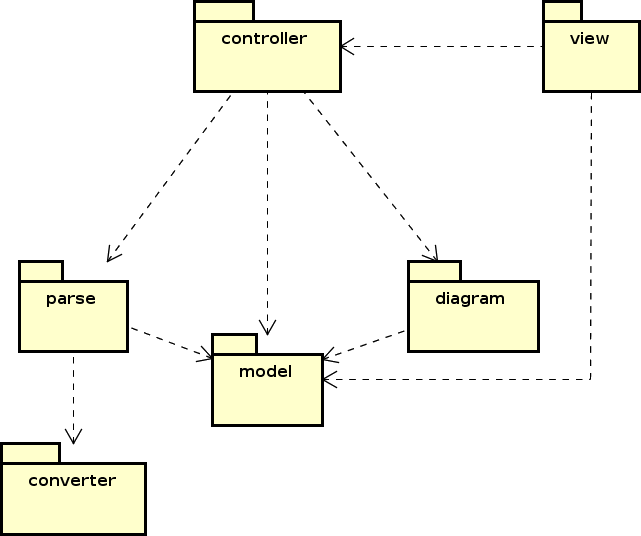
\includegraphics[scale=0.5]{img/ferramenta_arquitetura}
	\end{center}
\end{figure}
\subsubsection{Diagrama de Classes}\label{subsection:classes}
Na Figura \ref{figura:diagramaclasses} é apresentado o diagrama de classes, constituído das principais classes envolvidas na construção do software e suas relações. 

A classe Diagrama do pacote \textit{diagram} é utilizada para criar as conexões, pesquisar os elementos extraídos do arquivo SPEM e liga-los. A classe ParseXML é responsável pela extração dos elementos utilizados pela classe Diagrama. Esses elementos são extraídos seguindo a estrutura do arquivo SPEM gerado pela ferramenta EPF Composer. Essa estrutura está modelada no pacote model, onde as classes ContentElement, ContentPackage, MethodPackage, MethodLibrary e MethodPlugin representam as tags descritas no arquivo SPEM.
As classes Task, WorkProduct e Elemento são a estrutura no qual utilizamos para gerar o diagrama, onde o diagrama pode ser constituído de um conjunto de objetos instanciados de cada uma dessas classes. Por fim a classe DiagramaMBean é encarregada de controlar as requisições do usuário feitas nas páginas. Essa classe utiliza a tecnologia de gerenciamento de beans, no qual possibilita a ligação da interface com as páginas da visualização.

\begin{figure}[!htb]
	\caption{Diagrama de Classes}\label{figura:diagramaclasses}
	\begin{center}
		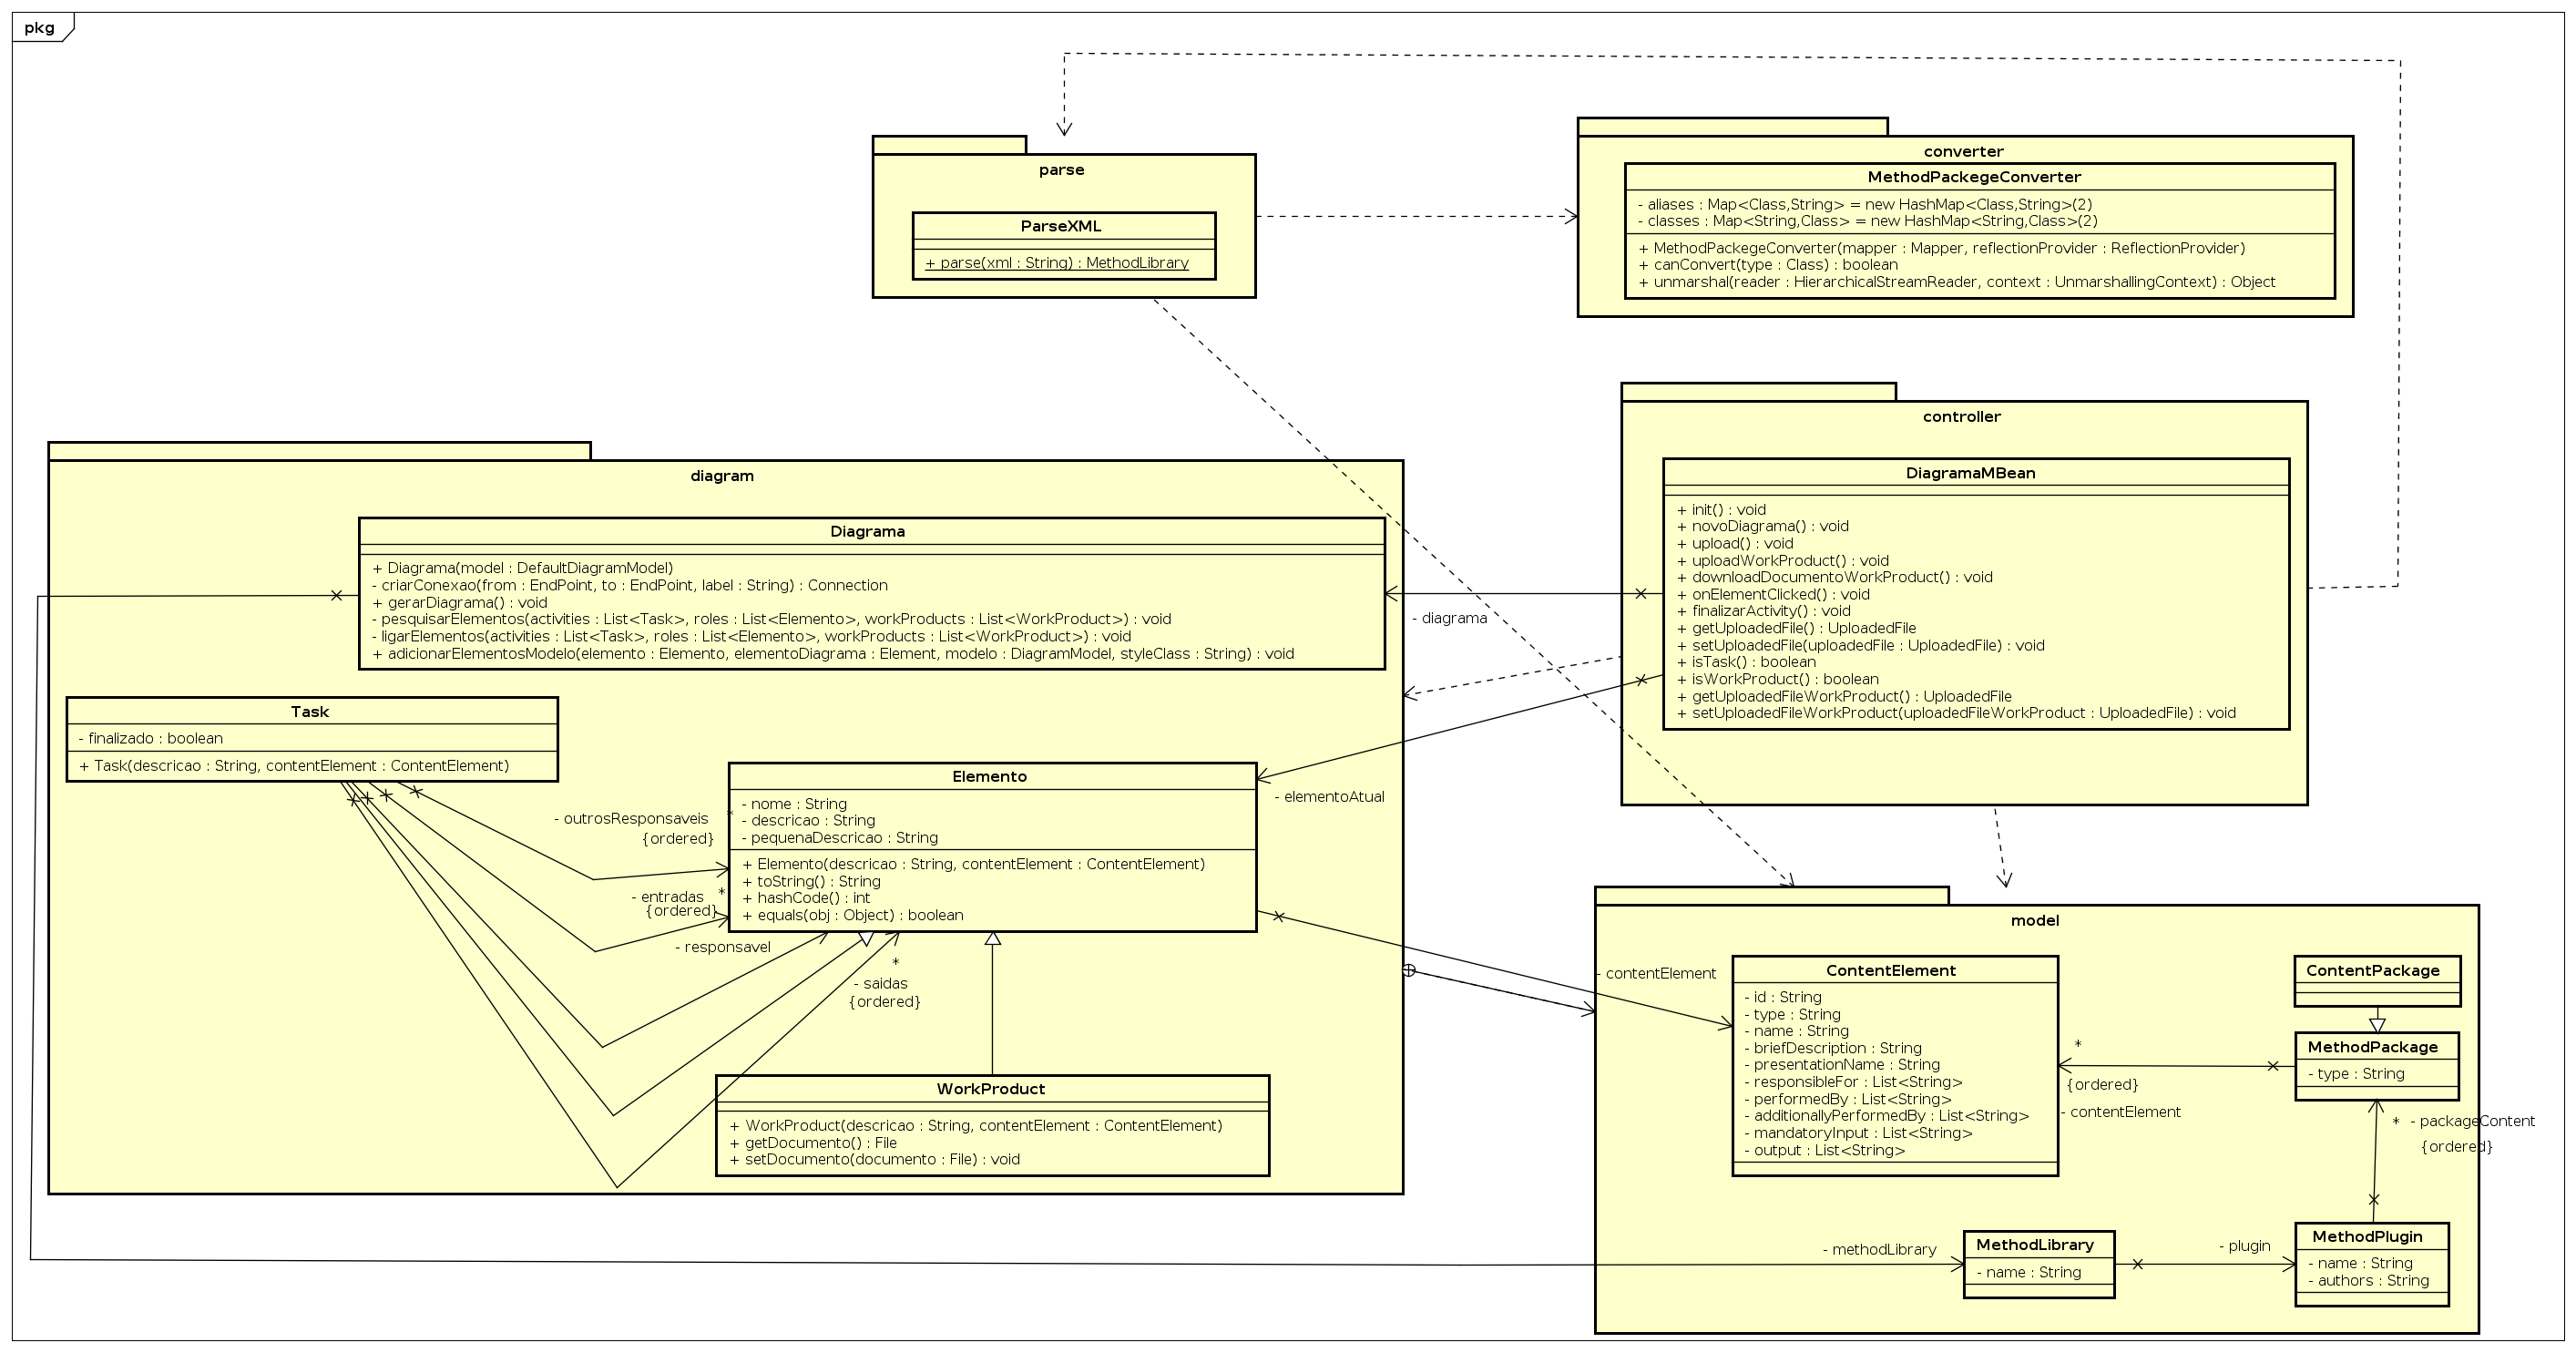
\includegraphics[scale=0.2]{img/ferramenta_diagrama_classes}
	\end{center}
\end{figure}


